\apendices

\partapendices

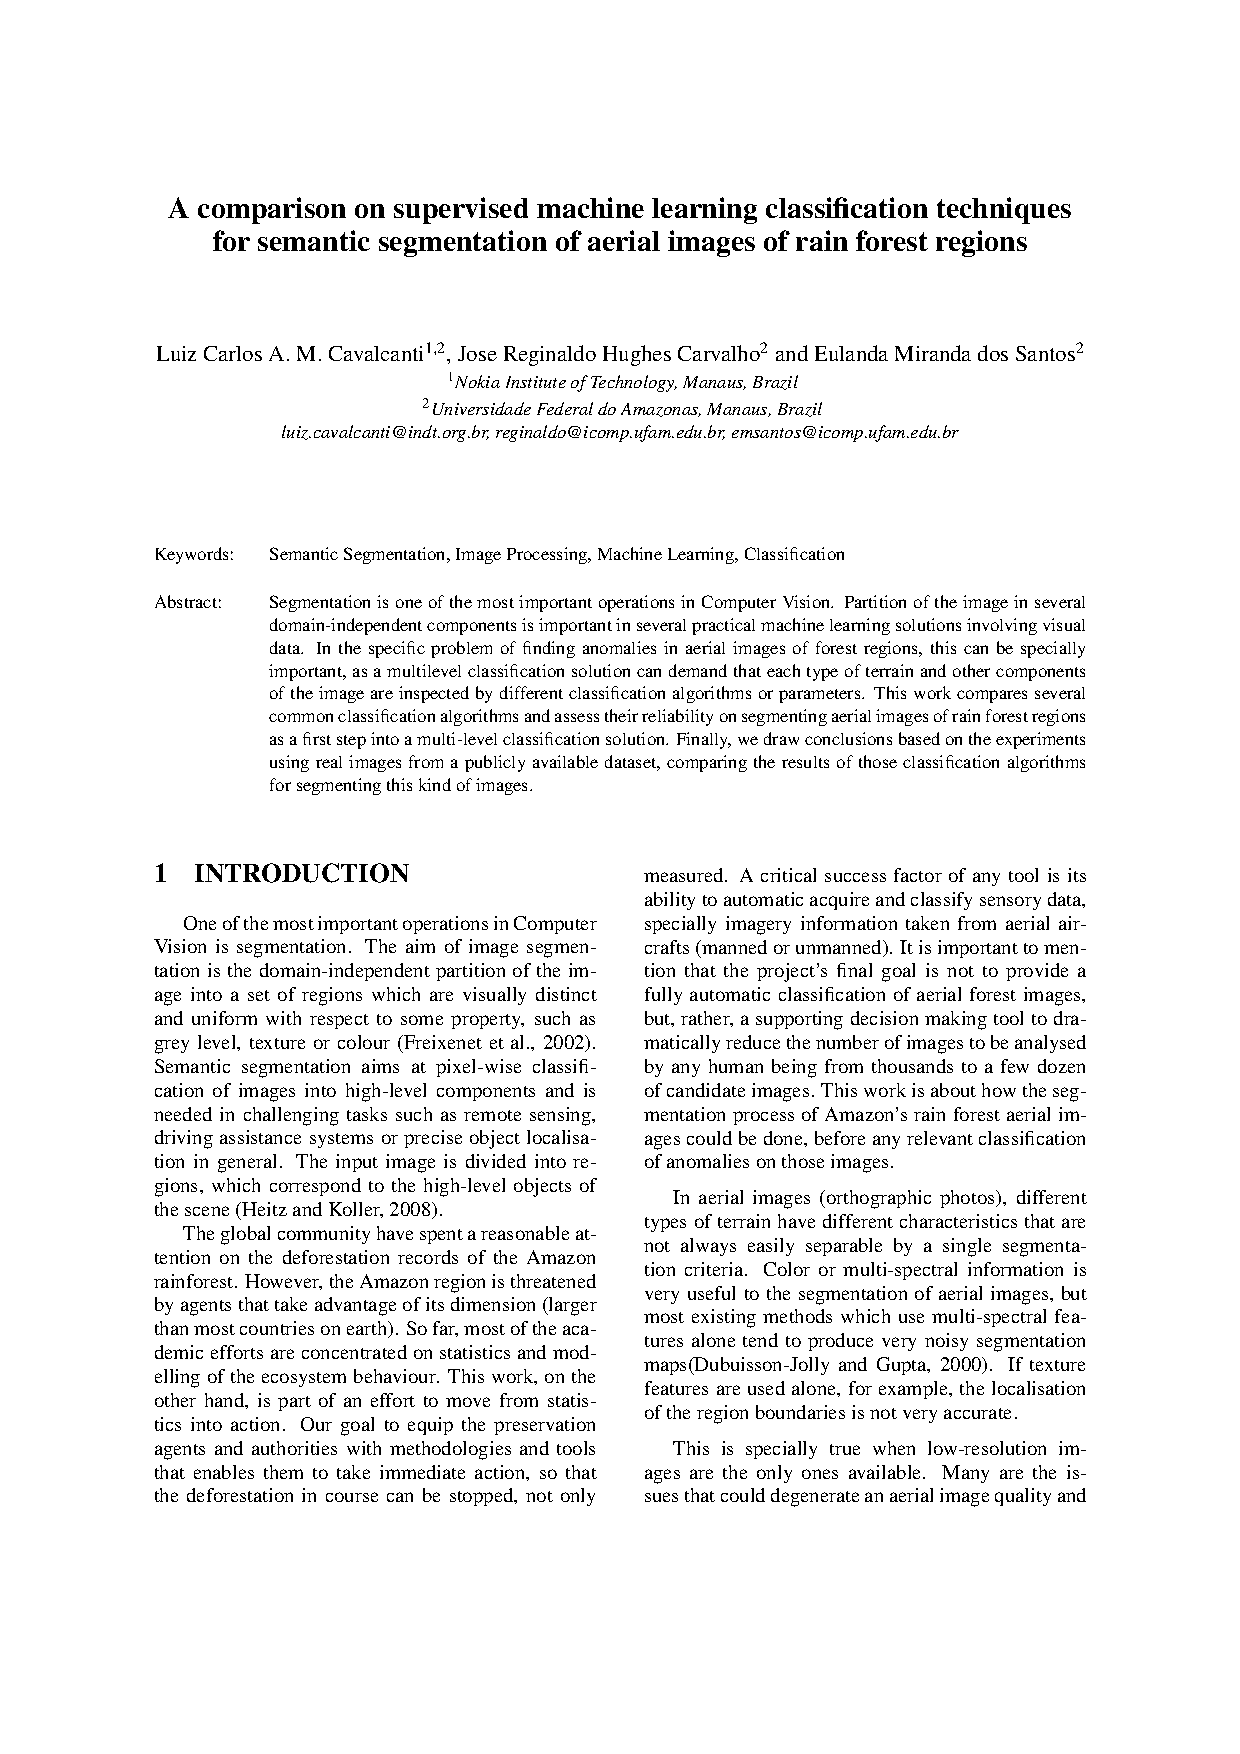
\includepdf[pages={-},addtotoc={1,chapter,1,A comparison on supervised machine learning classification techniques for semantic segmentation of aerial images of rain forest regions,cap:visapp2015}]{articles/visapp2015.pdf}

\chapter{Instruções da ferramenta de segmentação manual}\label{apendice:instrucoesManualSeg}
\section*{Objectives}

Segment aerial images on the Amazon rainforest according to terrain coverage/type

\section*{What are segments?}

Segments are closed regions on images that separate some elements in the image from the rest. Take figure 1, for example:

\begin{figure*}[h]
  \centering
  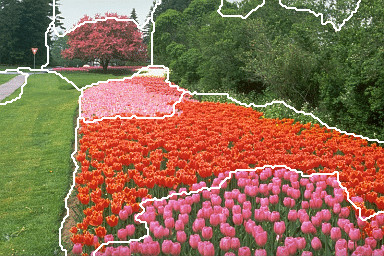
\includegraphics[width=0.7\textwidth]{imgs/manualseginstr_fig1}
  \legend{Fig. 1 - An image where parts of it were segmented}
\end{figure*}

This figure was divided in several segments. One could say that the person or algorithm segmented this image to separate different kinds of vegetation, other would argue that it was divided simply by dominant color. The point is that there is no correct or proper segmentation unless you know what are you trying to separate or analyse in the image.

Segmentations can also vary by granularity. Let's observe figure 2:

\begin{figure*}[h!]
  \centering
  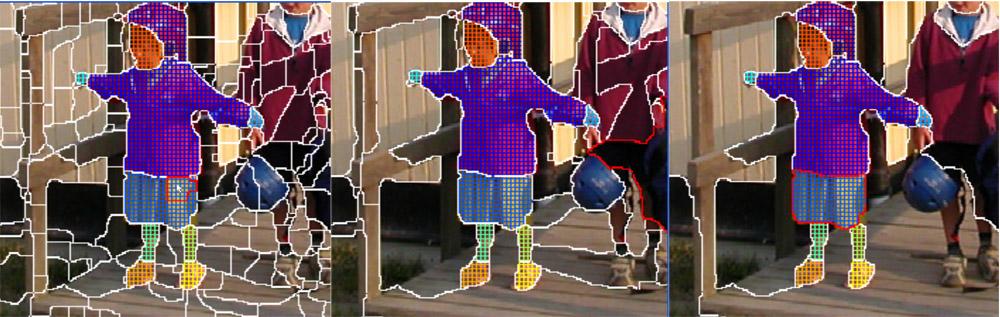
\includegraphics[width=0.9\textwidth]{imgs/manualseginstr_fig2}
  \legend{Fig. 2 - The same image segmented with different granularities}
\end{figure*}

\vspace{1in}

All those images segment the same image with seemingly the same valid criteria, but with different granularity. This is also perfectly normal in human or manual segmentation, since we tend to describe or view objects with different levels of detail.

\section*{What do you need to do?}

Your mission is to manually segment the given images as accurately as possible, according to your own judgment.

The criteria here is terrain coverage. So, we would like to separate different vegetations, geological formations and human-made objects. Let's have an example with figure 3:

\begin{figure*}[h!]
  \centering
  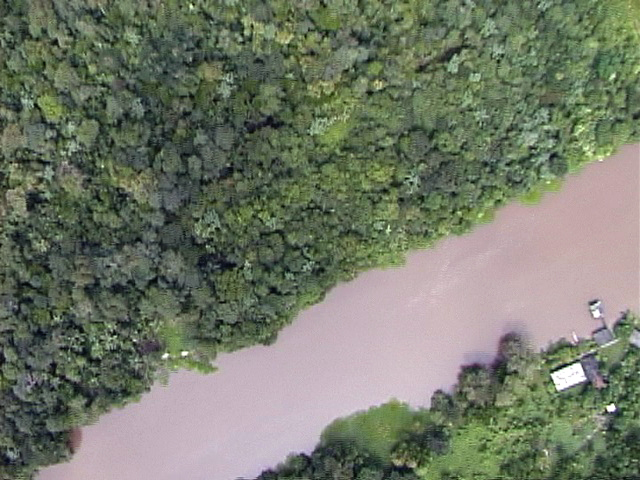
\includegraphics[width=0.45\textwidth]{imgs/manualseginstr_fig3a}
  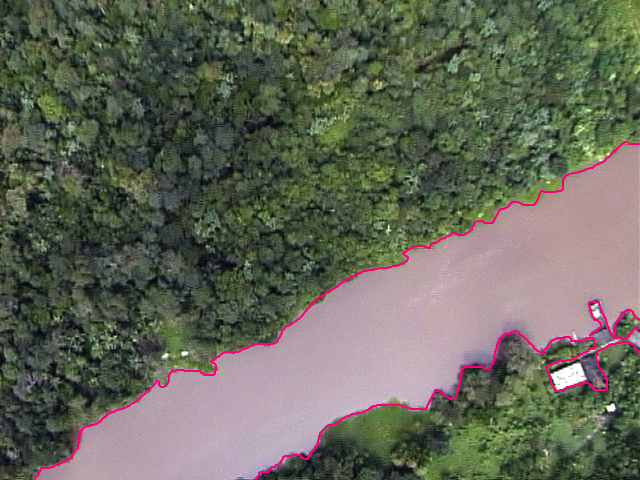
\includegraphics[width=0.45\textwidth]{imgs/manualseginstr_fig3b}
  \legend{Fig. 3 - An original image and a plausible segmentation for it, according to this experiment's criteria}
\end{figure*}


The pink/magenta line on the rightmost picture separates different types of terrain coverage and objects. An overly obsessed person would maybe segment every tree in the forest patch on that imagem, but that's not necessary.

If we look closer on the lower right corner, we can see several human-made structures. In this example, the person that segmented the image chose to put all buildings in a single segment. Other person would choose to define a segment for every individual building. None are wrong, they just decide to segment the image on a different granularity.

If an image is homogeneous, or in other words, if it has a single type of terrain/coverage, no segmentation is needed. An example of our dataset of that case is show in figure 4:


\begin{figure*}[h!]
  \centering
  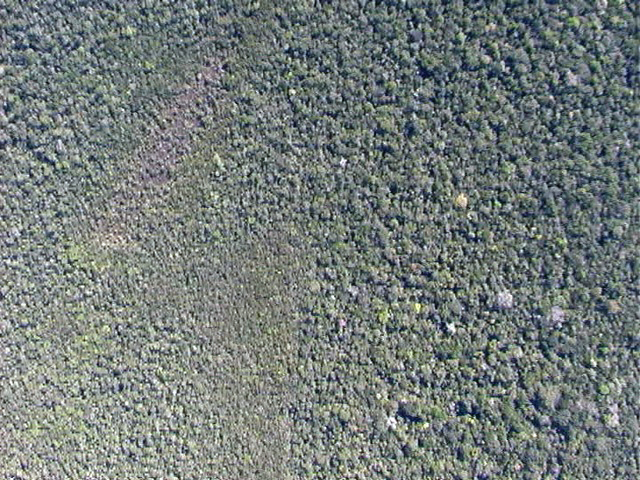
\includegraphics[width=0.7\textwidth]{imgs/manualseginstr_fig4}
  \legend{Fig. 4 - An homogeneous image. Makes little sense to segment it at all}
\end{figure*}

To help you segment the images in the experiment, a fairly simple tool is available. The following section describe how it works.

\section*{The segmentation tool}

As figure 5 shows, the segmentation tool interface is divided in two parts. The toolbar on the top, with all the commands necessary for the segmentation of the image, and the canvas on the bottom, where the user can actually segment the image.

\begin{figure*}[h!]
  \centering
  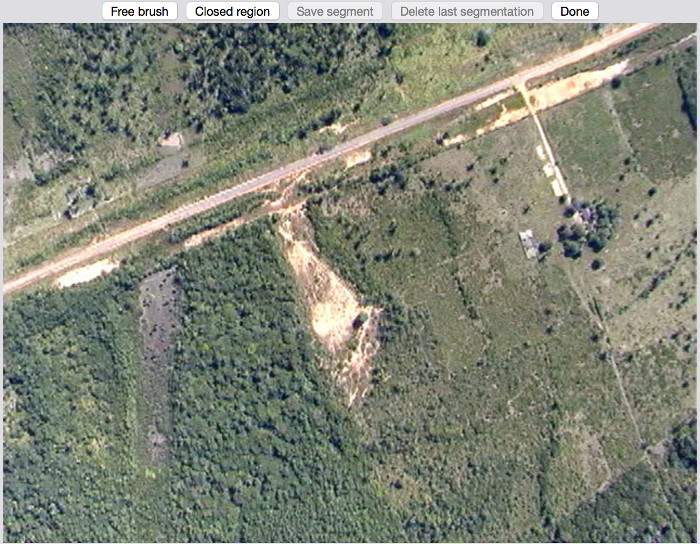
\includegraphics[width=0.7\textwidth]{imgs/manualseginstr_fig5}
  \legend{Fig. 5 - Segmentation tool interface}
\end{figure*}

When a new image is given, you must chose which drawing tool you will use. For segments that crosses the image from one edge to the other or subdivides previous segments, the "free brush" is the ideal tool. It allows you to draw freely on the canvas, defining the segment border as you go, describing an open-ended path (figure 6).

\begin{figure*}[h!]
  \centering
  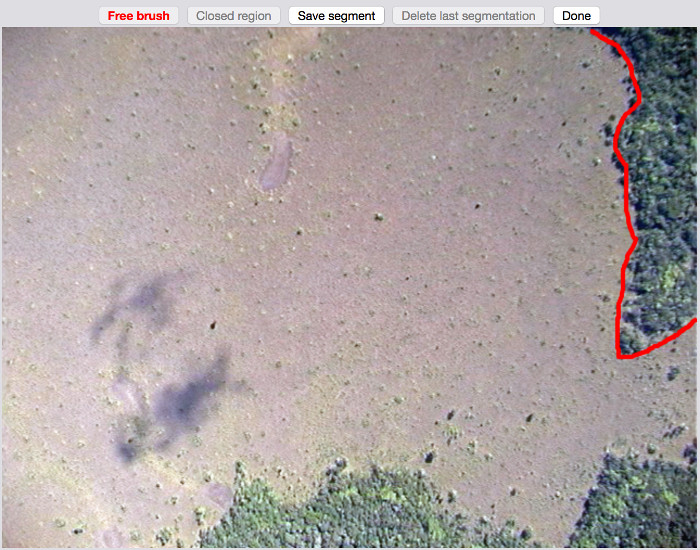
\includegraphics[width=0.7\textwidth]{imgs/manualseginstr_fig6}
  \legend{Fig. 6 - Using the "free brush" tool to draw an open-ended path}
\end{figure*}

The "closed region" tool, as the name implies, forces the drawn segment to be a closed on. It's ideal for internal segments of the image, those segments that don't collide with previous ones and don't touch the borders of the image (figure 7 shows an example).

\begin{figure*}[h!]
  \centering
  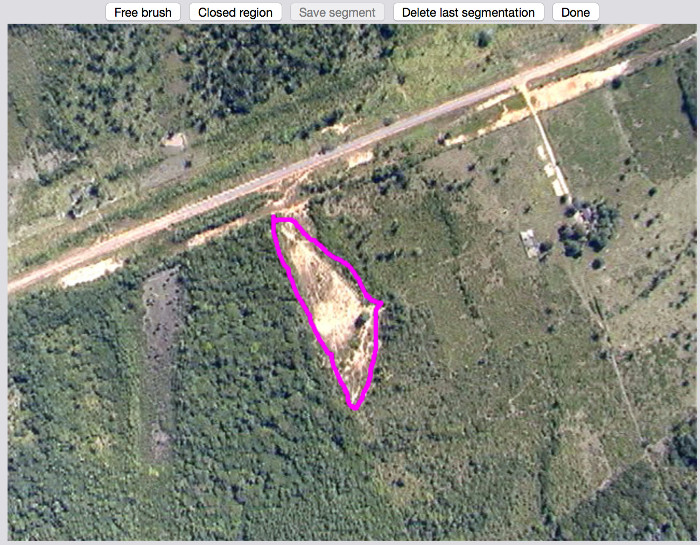
\includegraphics[width=0.7\textwidth]{imgs/manualseginstr_fig7}
  \legend{Fig. 7 - Using the "closed region" tool to determine a internal segment on the image}
\end{figure*}

For both drawing tools, you have two ways of interaction. You can draw continuously, as you would do in any computer-aided drawing tool, of you can just click on key point to create a path. Experiment on those two ways until you feel comfortable.

The previous strokes on the current region you are drawing can be undone by selecting the "undo" option.

After you create a segment, the next step is to select the "save segmentation" option. This registers the current segment and changes its colour. If there is more regions on the current image to segment, you can select a new segment type (closed region or free brush) and start drawing it right away.

If you feel that a previous segment was not adequate, you can click the "delete last segmentation" option. As the name implies, it will remove the last defined segment on the image. You can continue to use this option until there is no more defined segments on the current image.

Once you feel that the image is properly segmented, you should select the "done" option. A brief confirmation box will appear. If you are sure that the work in this image is done, you can confirm it. In this moment, all data regarding your segmentation will be sent to the experiment server and a new image will be shown.

We understand that manually segmenting images can be a tiresome process. If you feel tired, please stop. It's better to return when you feel refreshed and willing to help. You just need to use the same user identifier on the login page to pick the segmentation experiment where you left it.

\textbf{Thank you so much for your help. Try to have some good time :)}